\documentclass[12pt]{article}

%===================================================================================
% Paquetes
%----------------------------------------------------------
\usepackage{textcomp}
\usepackage[x11names,table]{color}
% \topmargin=-2cm
\usepackage{amsmath}
\usepackage{amsfonts}
\usepackage{amssymb}
\usepackage{latexsym}
\usepackage{graphicx}
\usepackage[T1]{fontenc}
\usepackage[latin1]{inputenc}
\usepackage{listings} \lstset {language = Python, basicstyle=\bfseries\ttfamily, keywordstyle = \color{blue}, commentstyle = \bf\color{gray}}
\usepackage{hyperref}
\usepackage{float}

% \textheight=20cm
% \textwidth=18cm
% \oddsidemargin=-1cm

\usepackage{xcolor}
% \textheight=27cm

% opening
\title{Proyecto de Simulaci\'on}
\author{Mauricio L. Perdomo Cort\'es. C-412}
% 
% 
\begin{document}
\vspace{8.cm}

\maketitle

\begin{center}
    Facultad de Matem\'atica y Computaci\'on\\\vspace{0.2cm} Universidad de La Habana
\end{center}

\clearpage

% \tableofcontents
\newpage

\section{Orden del Problema}
% \centering
\textsc{\textbf{L\'ogica Difusa:}}

La orden de nuestro trabajo se encuentra en un pdf que acompa\~na a este en el repositorio de GitHub.

\section{Ideas para la implemetaci\'on.}
En el proyecto est\'an creadas distintas clases y funciones que nos permiten reprsentar sistemas de inferencia difusa, contamos
con la definici\'on de variables lingu\'isticas a trav\'es de la clase LinguisticVar en la que podemos especificar el nombre, los t\'erminos, el dominio y 
las funciones de pertenecia de cada uno de sus t\'erminos (se ofrecen tambi\'en distintas funciones de pertenencia muy usadas como son triangular, trapezoidal, gamma y sig). 
Un sistema estar\'a definido por un grupo de variables de entrada (estado), un conjunto de variables de salida (control) y un conjunto de reglas definidas mediante la clase
SystemRule. La clase SystemRule representa las reglas del sistema conteniendo las variables que participan en el antecedente de la regla, las variables de salida que participan en las 
consecuencias de la regla y la regla como tal, definida mediante la clase FuzzyRule. La clase FuzzyRule est\'a conformada mediante un antecedente y un conjunto de consecuencias, estos antecendentes y consecuencias
son predicados definidos mediante la clase FuzzyFormula, estos predicados est\'an definidos por conjuntos difusos y operaciones l\'ogicas entre ellos, los conjuntos difusos se representan mediante la clase FuzzySet y est\'an definidos por un 
dominio y una funci\'on de pertenecia.

Una vez creado el sistema de inferencia, este puede inferir resultados mediante el m\'etodo de Mandami \'o el m\'etodo de Larsen, estos resultados son devueltos
en forma de diccionario, donde las llaves son las variables de salida(control) del sistema y y para cada una existe un conjunto difuso que representa la respuesta.
Para obtener valores espec\'ificos podemos utilizar alguno de los m\'etodos de desfusiciaci\'on que ofrecemos que son Mean of Maximun (mom), Smallest Maximun (som),
Largest Maximun (lom), Center of Area (coa), Bisector of Area (boa).

\section{Problema:}
\subsection{Planteamiento}
Debido a las medidas sanitarias acatadas como consecuencia del contagio de la Covid-19, el programa televisivo Masterchef Espa\~na no podr\'a emitir en la forma a la que estamos
acostumbrados. Para evitar el contacto entre concursantes y jueces el mejor aspirante de esta semana se decidir\'a mediante un cocinado particular. En este cocinado los participantes
utilizar\'an sus conocimientos desde sus casa mientras que los jueces estar\'an atentos a los detalles mediantes c\'amaras caseras instaladas por los mismo participantes. La prueba estar\'a dividida
en tres secciones, la primera ser\'a la elecci\'on del producto a cocinar, esta estapa ser\'a valorada por Pepe Rodr\'iguez; luego vendr\'a el proceso de elaboraci\'on del plato, que ser\'a valorado por Jordi Cruz y por \'ultimo 
el procedimiento de emplatado, que ser\'a valorado por Samantha Vallejo. Cada una de estas fases tendr\'a una valoraci\'on otorgada por los jueces y se nos ha pedido que creemos un sistema de inferencia difusa que podamos utilizar para definir
el ganador de la prueba.
\subsection{Soluci\'on}
Para resolver el problema definimos cuatro variables lingu\'isticas, las tres primeras ser\'an nuestras variables de estado y la \'ultima nuestra variable de control:
\begin{itemize}
	\item Calidad del Producto, esta variable esta compuesta por dos t\'erminos buena y excelente con las siguientes funciones de pertenencia
	\begin{figure}[H]
		\centering
		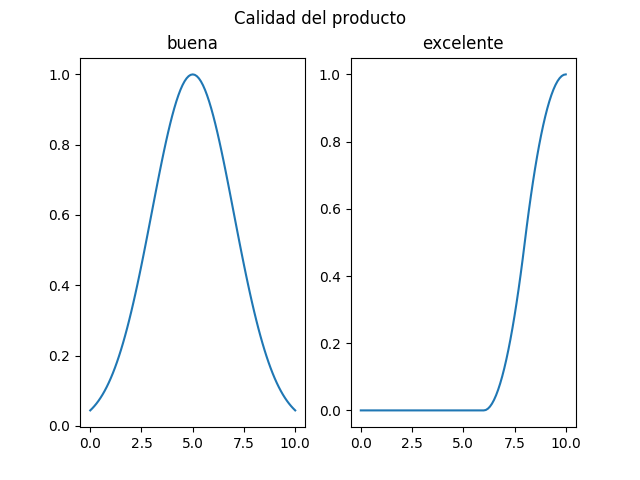
\includegraphics[width=0.8\linewidth, height=5cm ]{product.png}
	\end{figure}

	\item Calidad de la Elaboraci\'on, esta variable esta compuesta por tres t\'erminos mala, buena y excelente con las siguientes funciones de pertenencia
	\begin{figure}[!h]
		\centering
		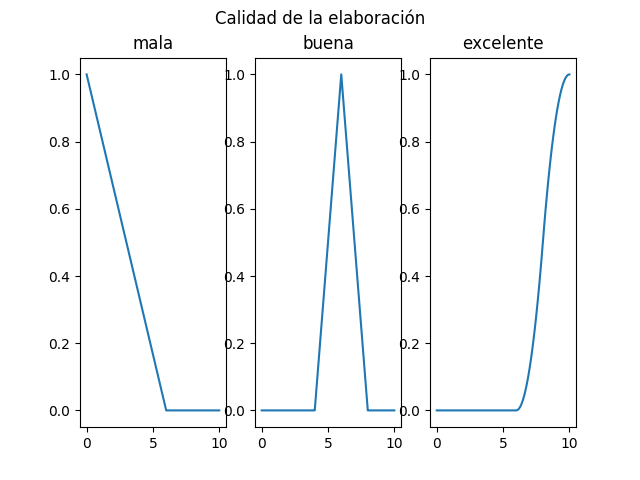
\includegraphics[width=0.9\linewidth, height=6cm ]{cook.png}
	\end{figure}

	\item Calidad del Emplatado, esta variable esta compuesta por tres t\'erminos malo, bueno y excelente con las siguientes funciones de pertenencia
	\begin{figure}[!h]
		\centering
		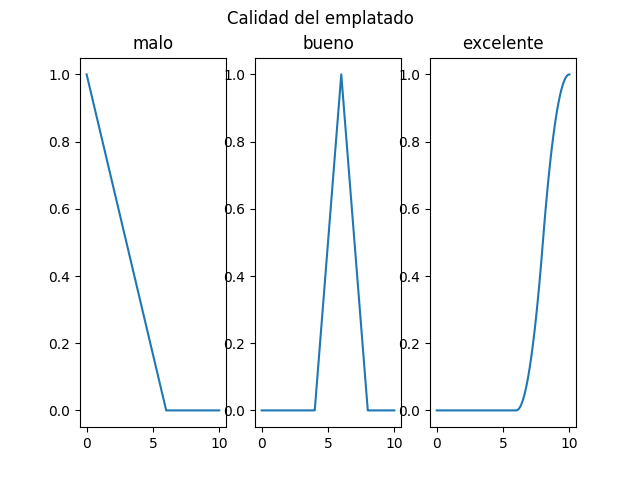
\includegraphics[width=0.9\linewidth, height=6cm ]{emplatado.png}
	\end{figure}
	\newline
	\newline
	\newline
	\newline
	\item Valoraci\'on, esta variable esta compuesta por tres t\'erminos mala, buena y excelente con las siguientes funciones de pertenencia
	\begin{figure}[!h]
		\centering
		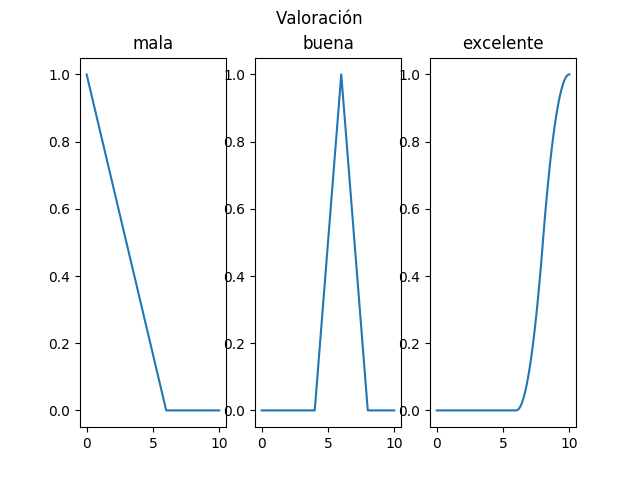
\includegraphics[width=0.9\linewidth, height=6cm ]{val.png}
	\end{figure}
\end{itemize}

Las reglas que rigen nustro sistema son:
\begin{itemize}
	\item Si la elaboraci\'on es \textbf{excelente} \textit{y} el emplatado es \textbf{excelente} entonces la valoraci\'on es \textbf{excelente}.
	\item Si la elaboraci\'on es \textbf{excelente} \textit{y} el emplatado es \textbf{malo} entonces la valoraci\'on es \textbf{buena}.
	\item Si la elaboraci\'on es \textbf{mala} entonces la valoraci\'on es \textbf{mala}.
	\item Si el producto es \textbf{excelente} \textit{y} la elaboraci\'on es \textbf{buena} \textit{y} el emplatado es \textbf{excelente} entonces la valoraci\'on es \textbf{excelente}.
	\item Si la elaboraci\'on es \textbf{buena} \textit{y} el emplatado es \textbf{malo} entonces la valoraci\'on es \textbf{mala}.
	\item Si el producto es \textbf{bueno} \textit{y} la elaboraci\'on es \textbf{excelente} \textit{y} el emplatado es \textbf{malo} entonces la valoraci\'on es \textbf{buena}.
	\item Si la elaboraci\'on es \textbf{buena} \textit{y} el emplatado es \textbf{bueno} entonces la valoraci\'on es \textbf{buena}.
\end{itemize}

Teniendo preparado el sistema anteriormente descrito y con las siguientes puntuaciones de los concursantes:
\newline
\newline
\newline
\begin{table}
	\begin{center}
		\begin{tabular}{| l | l | l | l |}
			\hline
			Participante & Producto & Elaboraci\'on & Emplatado\\
			\hline
			Nico & 8 & 9 & 8\\
			\hline
			Josy & 7 & 7 & 8\\
			\hline
			Terre & 6 & 6.6 & 5\\
			\hline
			Flo & 6 & 4.5 & 4.8\\
			\hline
		\end{tabular}
		
	\end{center}
	
\end{table}
\newline
Se obtienen las siguientes valoraciones:
\newline
\begin{table}[H]
	\begin{center}
		\begin{tabular}{| l | l |}
			\hline
			Participante & Valoraci\'on\\
			\hline
			Nico & 9.0\\
			\hline
			Josy & 8.5 \\ 
			\hline
			Terre & 6.0 \\
			\hline
			Flo & 3.8 \\  
			\hline
		\end{tabular}
		
	\end{center}
	
\end{table}

Y el ganador de la semana es \textbf{Nico}.

\section{GitHub link al c\'odigo del proyecto}
\href{https://github.com/stdevMauricio1802/fuzzy-inference-system.git}{C\'odigo Fuente}
\end{document}